\documentclass[nonacm=true, language=german]{acmart}

\usepackage{booktabs}
\usepackage{makecell}

\usepackage{dirtytalk}
\usepackage{nameref}
\usepackage{acronym}
\usepackage{svg}

\usepackage{tikz}
\usetikzlibrary{graphs}

\tikzstyle{node} = [minimum height=1.5cm, minimum width=3cm, text centered, align=center, rounded corners, fill=blue!30]

%\setcounter{tocdepth}{3}

\newcommand{\tabitem}{~~\llap{\textbullet}~~}

\title{Network Simulation}

\subtitle{Zusammenfassung}

\author{Per Natzschka}

\email{per.natzschka1@mailbox.tu-dresden.de}

\date{today}

\begin{document}

\maketitle

\tableofcontents

\section*{Abkürzungen}
\begin{acronym}
    \acro{DES}{Discrete-Event Simulation}
    \acro{PMF}{Probability Mass Function}
    \acro{CDF}{Cumulative Distribution Function}
    \acro{PDF}{Probability Density Function}
\end{acronym}

\newpage

\section{Network Simulation}

\subsection{Systemuntersuchung}

\begin{figure}[ht]
    \centering
    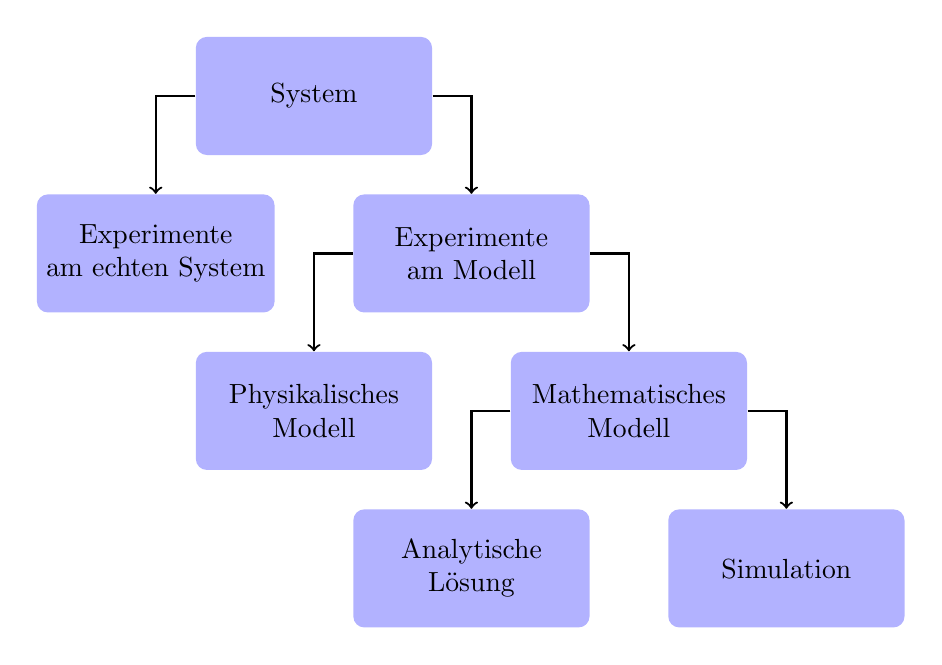
\begin{tikzpicture}
    \matrix[row sep=0.5cm, column sep=-1cm] {
        & \node[node](1){System}; \\
        \node[node](21){Experimente \\ am echten System}; & & \node[node](22){Experimente \\ am Modell}; \\
        & \node[node](31){Physikalisches \\ Modell}; & & \node[node](32){Mathematisches \\ Modell}; \\
        & & \node[node](41){Analytische \\ Lösung}; & & \node[node](42){Simulation}; \\
        }; 
        
        \graph {
            (1) ->[to path={-| (\tikztotarget)}, thick] (21);
            (1) ->[to path={-| (\tikztotarget)}, thick] (22);
            (22) ->[to path={-| (\tikztotarget)}, thick] (31);
            (22) ->[to path={-| (\tikztotarget)}, thick] (32);
            (32) ->[to path={-| (\tikztotarget)}, thick] (41);
            (32) ->[to path={-| (\tikztotarget)}, thick] (42);
        };
    \end{tikzpicture}
    \caption{Möglichkeiten der Systemuntersuchung}
    \label{fig:ways_study}
\end{figure}

\begin{itemize}
    \item Experimente am echten System
    \begin{itemize}
        \item teuer
        \item System existiert möglicherweise nicht
    \end{itemize}
    \item Experimente am physikalischen Modell
    \begin{itemize}
        \item untypisch bei Netzwerksimulationen
        \item begrenzte Einsicht durch Feldtests
    \end{itemize}
    \item Analytische Lösung eines Mathematischen Modells
    \begin{itemize}
        \item zu präferieren
        \item Modelle schnell zu komplex
        \item hohe Abstraktion nötig
    \end{itemize}
    \item Simulation
    \begin{itemize}
        \item letzter Ausweg
        \item Mittelweg zwischen Analytischer Lösung und Physikalischem Modell
    \end{itemize}
\end{itemize}

\subsection{Modelle}

\begin{itemize}
    \item Modell: Repräsentation eines Systems, um es zu untersuchen
    \item statisch/dynamisch
    \item deterministisch/stochastisch
    \item diskret/kontinuierlich
\end{itemize}

\subsection{Simulationen}

\subsubsection{Klassifikation von Simulationen}

\begin{itemize}
    \item Klassifikation abhängig von Modell
    \begin{itemize}
        \item statisch/dynamisch
        \item deterministisch/stochastisch
        \item diskret/kontinuierlich
    \end{itemize}
    \item \ac{DES}
    \begin{itemize}
        \item dynamisch, stochastisch, diskret
        \item trace-driven
        \item Objekt-/Prozessorientiert
        \item parallel/verteilt
    \end{itemize}
    \item Terminierende Simulationen
    \begin{itemize}
        \item spezifische Start- und Endbedingungen
        \item Messungen hängen von Start- und Endbedingungen ab
        \item ähnlich zu transienter Analyse (Impulsantwort)
        \item z. B. Simulation der Flugbahn eines fallenden Balles, bis er den Boden berührt
    \end{itemize}
    \item Steady-State Simulationen
    \begin{itemize}
        \item kein natürliches Event legt Simulationslänge fest
        \item überprüfen von Langzeitverhalten im eingeschwungenen Zustand
        \item korrespondiert zur Steady-State Analyse
        \item z. B. Simulation eines Gewichtes an einer Feder
    \end{itemize}
\end{itemize}

\subsubsection{Schritte einer Simulationsuntersuchung}

\begin{enumerate}
    \item Problemformulierung und Planung der Untersuchung
    \item Daten sammeln und Modelldefinition
    \item Validierung des konzeptuellen Modells
    \item Programmerstellung und Verifikation
    \item Testdurchläufe
    \item Validierung des programmierten Modells
    \item Experimente designen
    \item Simulation durchführen
    \item Output analysieren
    \item Dokumentieren, präsentieren, Ergebniss nutzen
\end{enumerate}

\subsubsection{Vor- und Nachteile}

\begin{itemize}
    \item Vorteile
    \begin{itemize}
        \item meist einzige Möglichkeit
        \item erlaubt Annäherung an Systemverhalten unter geplanten Bedingungen
        \item Vergleich unterschiedlicher Designs
        \item Kontrolle über Bedingungen
        \item erlaubt Zeitlupe/-raffung
    \end{itemize}
    \item Nachteile
    \begin{itemize}
        \item stochastische Modelle geben nur Schätzungen der wahren Charakteristika
        \item teuer und zeitaufwendig zu entwickeln
        \item lange Laufzeiten
        \item massenhafte Outputdaten und Animationen lassen Ergebnisse glaubwürdiger erscheinen als sie sind
    \end{itemize}
\end{itemize}

\subsubsection{Pitfalls}

\begin{itemize}
    \item ungenau definierte Objekte/unnötige Details
    \item Fehlkommunikation mit Management
    \item Fokus auf Programmierung (\say{nur eine Programmierübung})
    \item Zufälligkeit nicht einberechnet
    \item keine/falsche Daten gesammelt
    \item unpassende Simulationssoftware (undokumentierte Features?)
    \item Zweckentfremdung von Animation
    \item Outpudaten als die einzig wahre Antwort bewerten
\end{itemize}

\subsubsection{Aufbau von \ac{DES}}

\text{}

\begin{table}[ht]
    \centering
    \begin{tabular}{c|c|c}
        \toprule
        Objekt                  & Typ               & Beschreibung \\
        \midrule
        Systemzustand           & Variablenmenge    & beschreibt System zu bestimmten Zeitpunkt \\
        Simulationsuhr          & Variable          & gibt aktuelle Simulationszeit $t$ an \\
        Eventliste              & Liste             & enthält nächste Auftrittszeit je Eventtyp \\
        Statistische Zähler     & Variablenmenge    & enthält statistische Informationen \\
        Initialisierungsroutine & Subprogramm       & initialisiert Simulationsmodell bei $t=0$ \\
        Zeitablaufsroutine      & Subprogramm       & bestimmt nächstes Event und setzt $t$ auf dessen Eintrittspunkt \\
        Eventroutine            & Subprogramm       & updated Systemzustand, wenn bestimmtes Event auftritt \\
        Bibliotheksroutine      & Subprogramm       & \makecell{generiert zufällige Beobachtungen \\ aus Wahrscheinlichkeitsverteilungen} \\
        Berichtsgenerator       & Subprogramm       & \makecell{berechnet Schätzungen der gewünschten Messungen \\ und generiert daraus Bericht am Simulationsende} \\
        Hauptprogramm           & Subprogramm       & \makecell{startet Zeitablaufsroutine, um nächstes Event zu bestimmen \\ und gibt Kontrolle an entsprechende Eventroutine} \\
        \bottomrule
    \end{tabular}
    \caption{Elemente von \ac{DES}}
    \label{tab:elements_des}
\end{table}

\newpage

\subsubsection{Statistische Aspekte}

\begin{itemize}
    \item beobachtete Daten als Input
    \begin{itemize}
        \item trace-driven
        \begin{itemize}
            \item direkt und nahe an echtem System
            \item kann nur historische Inputs reproduzieren $\rightarrow$ unflexibel
        \end{itemize}
        \item empirische Verteilung
        \begin{itemize}
            \item Datenwerte als Verteilung interpolieren
            \item recht valide, einfach, recht direkt
            \item kann generierte Varianten begrenzen, schwer zu ändern
        \end{itemize}
        \item theoretische Verteilung
        \begin{itemize}
            \item an theoretische Verteilung anpassen
            \item kompakte Repräsentation mit wenigen Parametern, Daten werden \say{geglättet}
            \item eventuell schwer, passende Verteilung zu finden
        \end{itemize}
    \end{itemize}
    \item Verteilungsfindung
    \begin{enumerate}
        \item für Familie entscheiden (exponentiell, gamma, Weibull, \dots)
        \item Parameter schätzen (z. B. Maximum Likelihood Estimation)
        \item Repräsentativität bewerten (Diagramme, Test, \dots)
    \end{enumerate}
    \item Statistische Analyse
    \begin{itemize}
        \item Terminierende Simulationen
        \begin{itemize}
            \item $n$ unabhängige Wiederholungen
            \item selbe Startbedingungen
            \item selbe Endbedingungen
            \item unterschiedliche Zufallszahlen
            \item Verteilung der Mittelwerte bilden (Normalverteilungsannahme)
        \end{itemize}
        \item Steady-State Simulationen
        \begin{itemize}
            \item anfängliche Warm-Up-Phase (keine Messungen)
            \item Konvergenz gegen Steady State
            \begin{itemize}
                \item weiterhin schwankende, korrelierende Beobachtungen
                \item Simulation lang genug für festgelegte Präzision
            \end{itemize}
        \end{itemize}
    \end{itemize}
    \item Probleme
    \begin{itemize}
        \item Länge der Warm-Up-Phase
        \begin{itemize}
            \item Daumenregeln
            \item graphische Verfahren
            \item statistische Test
        \end{itemize}
        \item Analyse der korrelierenden Daten
        \begin{itemize}
            \item Endkriterien, um Simulation bei gewünschter Präzision zu beenden
            \item Umgang mit korrelierenden Daten
            \item konzeptuell: unabhängige Wiederholungen, Abschnittsmittel
            \item zudem: andere, komplizierte statistische Methoden
        \end{itemize}
    \end{itemize}
\end{itemize}

\newpage

\section{M/M/1 Queues}

\subsection{Aufbau}

\begin{figure}[ht]
    \centering
    \includesvg[inkscape=png]{Mm1_queue}
    \caption{Aufbau der M/M/1 Queue}
    \label{fig:mm1_queue}
\end{figure}

\begin{itemize}
    \item Kendalls Notation
    \item \textbf{M}
    \begin{itemize}
        \item \textbf{M}emoryless arrival
        \item exponentielle Verteilung der Zeit zwischen Ankünften $\rightarrow$ Poisson-Prozess
    \end{itemize}
    \item \textbf{M}
    \begin{itemize}
        \item \textbf{M}emoryless service time
        \item exponentielle Verteilung der Bearbeitungszeiten
    \end{itemize}
    \item \textbf{1}
    \begin{itemize}
        \item \textbf{1} Server
    \end{itemize}
\end{itemize}

\subsection{Messungen}

\begin{table}[ht]
    \centering
    \begin{tabular}{c|c}
        \toprule
        Messung                     & Beschreibung \\
        \midrule
        Mittlere Verzögerung $D$    & \makecell{Durchschnitt der Verzögerungen $ D_i = W_i + S_i $ \\ $W_i$ \dots Wartezeit, $S_i$ \dots Bearbeitungszeit} \\
        Mittlere Queuelänge $N$     & \makecell{Durchschnitt von $N(t)$ für $ t \rightarrow \infty $ \\ $N(t)$ \dots Anzahl Kunden im System} \\
        Auslastung $U$              & Durchschnittlicher Anteil der Zeit mit $ N(t) > 0 $ \\
        Durchsatz $X$               & Durchschnittliche Anzahl abgeschlossener Bearbeitungen pro Zeitschritt \\
        \bottomrule
    \end{tabular}
    \caption{Typische Messungen bei M/M/1 Queues}
    \label{tab:mm1_measures}
\end{table}

\newpage

\subsection{Analyse}

\begin{itemize}
    \item Darstellung als Markov-Kette mit kontinuierlicher Zeit
    \begin{itemize}
        \item Zustand $i$: Anzahl Kunden im System
        \item $i \rightarrow i+1$: Ankunftsrate $\lambda$
        \item $i \rightarrow i-1$: Bearbeitungsrate $\mu$
    \end{itemize}
    \item Zustandswahrscheinlichkeiten: $ \displaystyle \pi_n = \lim_{t \to \infty} P(N(t) = n) $
    \item Balancegleichungen
    \begin{itemize}
        \item $ \lambda \pi_0 = \mu \pi_1 $
        \item $ (\lambda + \mu) \pi_i = \lambda \pi_{i-1} + \mu \pi_{i+1} $
    \end{itemize}
    \item Lösung im eingeschwungenen Zustand
    \begin{itemize}
        \item $\rho = \frac{\lambda}{\mu}$
        \item $\pi_i = \rho^i \pi_0$
        \item $ \displaystyle \sum_{i=0}^\infty \pi_i = \sum_{i=0}^\infty \rho^i \pi_0 = \frac{1}{1-\rho} \pi_0 = 1 \Rightarrow \pi_0 = 1 - \rho \Rightarrow \pi_i = \rho^i (1 - \rho) $
        \item modifizierte geometrische Verteilung
    \end{itemize}
    \item Messungen
    \begin{itemize}
        \item Durchschnittliche Anzahl Kunden im System: $ E[N] = \frac{\rho}{1-\rho} $
        \item Durchschnittliche Anzahl Kunden in der Queue: $ E[N_q] = \frac{\rho^2}{1-\rho} $
        \item Little's Law: $ E[N] = \lambda E[T] $
        \begin{itemize}
            \item Im eingeschwungenen Zustand gilt für Durchsatz: $ X = \lambda $
            \item Durchschnittliche Verzögerung: $ E[T] = \frac{E[N]}{\lambda} = \frac{\frac{1}{\mu}}{1-\rho} $
            \item Durchschnittliche Wartezeit: $ E[W] = \frac{E[N_q]}{\lambda} = \frac{\frac{\rho}{\mu}}{1-\rho} $
        \end{itemize}
    \end{itemize}
    \item linear steigende Verzögerung bei niedrigem $U$
    \item unbegrenzte Verzögerung für $\rho = U \rightarrow 1$
\end{itemize}

\newpage

\section{Wahrscheinlichkeitstheorie}

\begin{itemize}
    \item Simulationen modellieren stochastische Prozesse
    \item statistische Mehoden nötig, um
    \begin{itemize}
        \item Wahrscheinlichkeitsverteilungen und deren Parameter zu finden (Input-Modellierung)
        \item Simulationsergebnisse zu analysieren
    \end{itemize}
\end{itemize}

\subsection{Grundlegendes}

\begin{table}[ht]
    \centering
    \begin{tabular}{c|c}
        \toprule
        Begriff             & Beschreibung \\
        \midrule
        Zufallsexperiment   & ein Prozess dessen Ergebnis nicht mit sicherheit feststeht \\
        Ergebnisraum $S$    & die Menge aller möglichen Ergebnisse eines Zufallsexperiments \\
        Ergebnis            & ein Element des Ergebnisraums $S$ \\
        Ereignis $A$        & eine Menge von Ergebnissen, $A \subseteq S$ \\
        \bottomrule
    \end{tabular}
    \caption{Grundbegriffe der Wahrscheinlichkeitstheorie}
    \label{tab:prob_terminology}
\end{table}

\begin{itemize}
    \item $ A \cap B = \emptyset \Rightarrow P(A \cup B) = P(A) + P(B) $
    \item $ P(A|B) = \frac{P(A \cap B)}{P(B)} $
    \item $ P(A|B) = P(A) \Leftrightarrow P(A \cap B) = P(A) \cdot P(B) \Leftrightarrow A \text{ und } B \text{ unabhängig} $
\end{itemize}

\subsection{Zufallsgrößen und deren Verteilung}

\begin{itemize}
    \item Zufallsgröße: $ X: S \to \mathbb{R}_0^+ $
    \item diskrete Zufallsgröße: $ |X(S)| \leq |\mathbb{N}| $
    \begin{itemize}
        \item Wahrscheinlichkeitsfunktion/\ac{PMF}
        \begin{itemize}
            \item $ p_i = P(X = x_i) $
        \end{itemize}
        \item Verteilungsfunktion/\ac{CDF}
        \begin{itemize}
            \item $ \displaystyle F(x) = P(X \leq x) = \sum_{x_i \leq x} p_i $
            \item $0 \leq F(x) \leq 1$
            \item $F(x)$ monoton steigend ($x_1 \leq x_2 \Rightarrow F(x_1) \leq F(x_2)$)
            \item $ \displaystyle \lim_{x \to -\infty} F(x) = 0 $, $ \displaystyle \lim_{x \to +\infty} F(x) = 1 $
            \item $F(x)$ ist rechtskontinuierlich ($ \displaystyle \lim_{x \to x_0+} f(x) = f(x_0) $)
        \end{itemize}
    \end{itemize}
    \item kontinuierliche Zufallsgröße: $ |X(S)| > |\mathbb{N}| $
    \begin{itemize}
        \item \ac{CDF} gleich definiert 
        \item Dichtefunktion/\ac{PDF}
        \begin{itemize}
            \item $f(x) = \frac{d}{dx} F(x)$
            \item Verteilung der Wahrscheinlichkeiten über Werte der Zufallsgröße
            \item $ \displaystyle \int_a^b f(x) dx = P(a \leq X \leq b) $
        \end{itemize}
    \end{itemize}
\end{itemize}

\newpage

\subsection{Momente und Quantile}

\begin{itemize}
    \item \ac{CDF} $F(x)$ und \ac{PDF} definieren Zufallsgröße vollständig
    \item Funktionen aber oft zu komplex
    \item wenige Zahlen besser zur Beschreibung
\end{itemize}

\subsubsection{Erwartungswert}

\begin{itemize}
    \item Erwartungswert $m = E[X]$
    \item Berechnung
    \begin{itemize}
        \item $X$ diskret: $ \displaystyle E[X] = \sum_{i=1}^\infty x_i p_i $
        \item $X$ kontinuierlich: $ \displaystyle E[X] = \int_{-\infty}^\infty x f(x) dx $
    \end{itemize}
    \item Linearität: $ E[aX + bY] = a E[X] + b E[Y] $
    \item Funktion einer Zufallsvariable, $Y = g(X)$
    \begin{itemize}
        \item $X$ diskret: $ \displaystyle E[Y] = E[g(X)] = \sum_{i=1}^\infty g(x_i)p_i $
        \item $X$ kontinuierlich: $ \displaystyle E[Y] = E[g(X)] = \int_{-\infty}^\infty g(x)f(x) dx $
    \end{itemize}
\end{itemize}

\subsubsection{Varianz}

\begin{itemize}
    \item Varianz $\sigma^2 = Var[X]$
    \item $ Var[X] = E[(X - E[X])^2] = E[X^2] - E[X]^2 $
    \item Standardabweichung $\sigma$
    \item Eigenschaften
    \begin{itemize}
        \item $ Var[aX] = a^2 Var[X] $
        \item $ Var[X + Y] = Var[X] + Var[Y] $ (wenn $X$ und $Y$ unabhängig sind)
    \end{itemize}
\end{itemize}

\subsubsection{Momente}

\begin{itemize}
    \item Moment n-ter Ordnung: $ E[X^n], n \geq 1 $
    \item Zentrales Moment n-ter Ordnung: $ E[(X - E[X])^n], n \geq 1 $
    \item Beispiele
    \begin{itemize}
        \item Moment 1. Ordnung: Erwartungswert
        \item Zentrales Moment 2. Ordnung: Varianz
        \item Moment 3. Ordnung: Schiefe (Maß für Asymmetrie)
    \end{itemize}
    \item Verteilung kann auch durch Reihe von Momenten definiert werden (wenn diese existiert)
\end{itemize}

\newpage

\subsubsection{Median}

\begin{itemize}
    \item kleinster Wert $x_{0.5}$, sodass $F(x_{0.5}) \geq 0.5$
    \item alternative Möglichkeit, Mittelwert anzugeben
    \item kann sinnvoll sein, wenn Verteilung extreme Werte annehmen kann
\end{itemize}

\subsubsection{Quantile}

\begin{itemize}
    \item für $0 < q < 1$ ist das $q$-Quantil der kleinste Wert $x_q$, sodass $F(x) \geq q$
    \item wenn $X$ kontinuierlich und $F(x)$ streng monoton steigend: $F(x_q) = q, x_q = F^{-1}(q)$
    \item Median ist 0.5-Quantil
\end{itemize}

\subsection{Verteilungen}

\subsubsection{Geometrische Verteilung}

\begin{itemize}
    \item Experiment: Wiederhole Bernoulli-Versuche, bis zum ersten Erfolg
    \item Zufallsvariable: Anzahl an Versuchen
    \item \ac{PMF}: $ p_i = p(1 - p)^{i-1} $
    \item \ac{CDF}: $ \displaystyle F(i) = \sum_{j=1}^i p_j = 1 - (1 - p)^i $
    \item Erwartungswert: $ \displaystyle E[i] = \sum_{j=1}^\infty j p_j = \frac{1}{p} $
\end{itemize}

\subsubsection{Exponentialverteilung}

\begin{itemize}
    \item \ac{PDF}: $ f(x) = \lambda e^{-\lambda x}, x \geq 0 $
    \item \ac{CDF}: $ F(x) = 1 - e^{-\lambda x} $
    \item einziger Parameter: Rate $\lambda$
    \item Erwartungswert: $ \displaystyle E[X] = \int_{0}^\infty x \lambda e^{-\lambda x} dx = \frac{1}{\lambda} $
    \item Varianz: $ \displaystyle Var[X] = \int_{0}^\infty (x - \frac{1}{\lambda})^2 \lambda e^{-\lambda x} dx = \frac{1}{\lambda^2} $
\end{itemize}

\subsubsection{Normalverteilung}

\begin{itemize}
    \item \ac{PDF}: $ f(x) = \frac{1}{\sigma \sqrt{2 \pi}} e^{-\frac{1}{2} (\frac{x - \mu}{\sigma})^2} $
    \item \ac{CDF} hat keine geschlossene Form
    \item Notation: $ X \sim N(\mu, \sigma^2) $
    \item Standardnormalverteilung: $ Z \sim N(0, 1) $
    \item Projektion: $ F_X(x) = F_Z(\frac{x - \mu}{\sigma}) $
\end{itemize}

\newpage

\subsection{Hypothesentests}

\subsubsection{Statistische Hypothese}

\begin{itemize}
    \item Behauptung, die eine oder mehrere Populationen betrifft
    \item Verifikation nur durch Betrachtung der gesamten Population (bei Simulationen unmöglich)
    \item Falsifizierung
    \begin{itemize}
        \item Beweis durch Gegenbeispiel
        \item Folgt aus hoher Wahrscheinlichkeit $\rightarrow$ Hypothesentest
    \end{itemize}
\end{itemize}

\subsubsection{Vorgehen}

\begin{itemize}
    \item Vorgehen
    \begin{enumerate}
        \item Beginn bei originaler Hypothese (Alternativhypothese $H_1$)
        \item Logisches Komplement (Nullhypothese $H_0$) formulieren
        \item $H_0$ widerlegen
        \item Aus Falsifizierung von $H_0$ folgt Verifikation von $H_1$
    \end{enumerate}
    \item Folgerungen
    \begin{enumerate}
        \item $H_0$ widerlegt
        \begin{itemize}
            \item ausreichend Hinweise in Daten
            \item Wahrscheinlichkeit für Wahrheit von $H_0$ unter gewählter Grenze $\alpha$ (z. B. $\leq 5\%$)
            \item $H_0$ ablehnen ist nach Konstruktion äquivalent zum annehmen von $H_1$
        \end{itemize}
        \item $H_0$ nicht widerlegt
        \begin{itemize}
            \item durch nicht ausreichende Hinweise in Daten
            \item sicherer bei $H_0$ zu bleiben (\say{sicherer Standardfall})
        \end{itemize}
    \end{enumerate}
\end{itemize}

\subsubsection{Varianten}

\begin{itemize}
    \item One-/Two-Sample
    \begin{itemize}
        \item Test, ob Mittelwert einer Population von einem gegebenen Wert abweicht (one-sample)
        \item Test, ob sich zwei Populationen unterscheiden (two-sample)
    \end{itemize}
    \item Unpaired/paired two-sample
    \begin{itemize}
        \item paired Tests sind statistisch aussagekräftiger
        \item anwendbar, wenn Proben aus A und B abhängig sind
        \item z. B. bei Vorher-Nachher Vergleichen desselben Gebiets
    \end{itemize}
    \item Normal-/Unnormal verteilte Daten
    \begin{itemize}
        \item bei Normalverteiltungen (oder Zentraler Grenzwertsatz): t-Test
        \item sonst: Wilcox-Test (weniger aussagekräftig)
    \end{itemize}
\end{itemize}

\newpage

\section{Validierung}

\begin{itemize}
    \item Konzeptuelle Validierung: Überprüfung des konzeptuellen Modells
    \begin{itemize}
        \item Sind die Abstraktionen, Vereinfachungen, Annahmen des Modells korrekt?
        \item Bauen wir das richtige Modell?
        \item Problem: Absolute Validation zu teuer
    \end{itemize}
    \item Verifikation: Überprüfung der Implementation
    \begin{itemize}
        \item Ist die Implementation korrekt (sprich: bugfrei)?
        \item Bauen wir das Modell richtig?
        \item Problem: Algorithmisch nicht lösbar (Halteproblem)
    \end{itemize}
    \item keine Garantien für Validität möglich
    \item Tests durchführen, bis man sicher genug ist
\end{itemize}

\subsection{Durchführende}

\begin{itemize}
    \item Modellentwickler
    \item Modellnutzer (geleitet durch Entwickler)
    \item Dritte (während oder nach Entwicklung)
    \item Bewertungsmodell
    \begin{itemize}
        \item Subjektive Punkte für verschiedene Validierungsaspekte
        \item Kombination von Einzel-, Kategorie- und Gesamtbewertungen
        \item Schwächen
        \begin{itemize}
            \item Bestandspunktzahl ist subjektiv
            \item kein guter Indikator für Korrektheit
            \item kann zu hohes Vertrauen in Modell verursachen
        \end{itemize}
    \end{itemize}
\end{itemize}

\subsection{Schritte}

\begin{itemize}
    \item Datenvalidität
    \begin{itemize}
        \item ausreichend, genau
        \item Umformungen korrekt (z. B. dB $\leftrightarrow$ lineare Skala)
        \item Außenseiter finden und auf Korrektheit überprüfen
    \end{itemize}
    \item Konzeptuelle Modellvalidierung (z. B. Linearität, Unabhängigkeit von Prozessen)
    \item Computergestützte Modellverifikation
    \begin{itemize}
        \item Korrektheitsbeweise
        \item Struktur überprüfen
    \end{itemize}
    \item Funktionelle Validität
    \begin{itemize}
        \item Simulationsdaten mit echtem System vergleichen (\nameref{tab:validation_operational})
    \end{itemize}
\end{itemize}

\begin{table}[ht]
    \centering
    \begin{tabular}{c|c c}
        \toprule
                    & beobachtbares System          & nicht-beobachtbares System \\
        \midrule
         subjektiv  & \makecell{
             \tabitem graphische Anzeigen \\
             \tabitem Modellverhalten erforschen
         }          & \makecell{
             \tabitem Vergleich zu anderen Modellen \\
             \tabitem Modellverhalten erforschen
         } \\
         objektiv   & \tabitem statistische Tests   & \makecell{\tabitem Vergleich zu anderen Modellen \\ durch statistische Tests} \\
         \bottomrule
    \end{tabular}
    \caption{Vergleich der Validationsmöglichkeiten der Funktionalität}
    \label{tab:validation_operational}
\end{table}

\newpage

\subsection{Techniken}

\subsubsection{Sehr typisch}
\begin{itemize}
    \item Animation
    \item Vergleich zu anderen Modellen
    \begin{itemize}
        \item einfache Fälle: analytische Modelle
        \item sonst: Ergebnisse anderer  (validierter) Modelle (z. B. aus anderen Simulationsframeworks)
    \end{itemize}
    \item Degenerate Tests
    \begin{itemize}
        \item Input- und interne Parameter auf degenerierende Fälle setzen
        \item z. B. $\lambda > \mu \Rightarrow$ monoton steigende Verzögerung
    \end{itemize}
    \item Ereignisvalidität
    \begin{itemize}
        \item Auftritt von Simulationsevents mit echten Events vergleichen
    \end{itemize}
\end{itemize}

\subsubsection{Typisch}

\begin{itemize}
    \item Test bei Extrembedingungen
    \begin{itemize}
        \item Ausgabe sollte für jede Kombination extremer/unwahrscheinlicher Faktoren plausibel sein
        \item z. B. es kommt lange kein Kunde an $\Rightarrow$ die Queue leert sich
    \end{itemize}
    \item Augenscheinvalidität
    \begin{itemize}
        \item Experten fragen, ob Modellstruktur und Ausgabe Sinn ergeben
    \end{itemize}
    \item Historische Datenvalidation
    \begin{itemize}
        \item trace-driven Simulation nutzen, um mit echtem System zu vergleichen
    \end{itemize}
    \item Parametervariabilitäts-Sensibilitäts Analyse
    \begin{itemize}
        \item Parameter variieren, um Effekt auf Ausgabe zu bestimmen
        \item selbe Effekte sollten bei echtem System auftreten
        \item für sensible Parameter: auf ausreichende Genauigkeit achten
    \end{itemize}
\end{itemize}

\subsubsection{Selten}

\begin{itemize}
    \item Funktionelle Grafiken
    \begin{itemize}
        \item Graphen von Leistungsmessungen während der Modellläufe anzeigen
    \end{itemize}
    \item Voraussagende Validierung
    \begin{itemize}
        \item Modell nutzen, um Systemverhalten vorauszusagen und dann vergleichen (Feldtest)
    \end{itemize}
    \item Turing-Test
    \begin{itemize}
        \item Experten fragen, ob er zwischen System- und Modellausgaben unterscheiden kann
    \end{itemize}
\end{itemize}

\newpage

\subsubsection{Untypisch}

\begin{itemize}
    \item Interne Validität
    \begin{itemize}
        \item mehrere Replikationen erstellen, um stochastische Varianz im Modell zu bestimmen
    \end{itemize}
    \item Historische Methoden
    \begin{itemize}
        \item Rationalismus: Annahmen als wahr annehmen $\rightarrow$ Modell durch logische Schlüsse bilden
        \item Empirismus: Annahmen und Ergebnisse empirisch validieren
    \end{itemize}
    \item Positive Ökonomie
    \begin{itemize}
        \item Modell muss Zukunft voraussagen können
        \item Annahmen und Modellstruktur nicht relevant
    \end{itemize}
    \item Multistate Validierung
    \begin{itemize}
        \item Kombination von Rationalismus, Empirismus und Positiver Ökonomie
    \end{itemize}
\end{itemize}

\subsection{Empfohlenes Vorgehen}

\begin{itemize}
    \item Animationen nutzen, um Systemzustand zu visualisieren
    \item Live-Graphen in GUI nutzen
    \item Degenerate Tests (z. B. Overload)
    \item Parametersensibilität testen
    \item Vergleich mit anderen Implementationen
    \item Augenscheinvalidierung des konzeptuellen Modells
    \item Modulweises Debugging
\end{itemize}

\end{document}